% Created 2025-02-20 Thu 16:48
% Intended LaTeX compiler: pdflatex
\documentclass[a4paper,12pt]{article}
\usepackage[utf8]{inputenc}
\usepackage[T1]{fontenc}
\usepackage{amsmath}
\usepackage{amssymb}
\usepackage{capt-of}
\usepackage{hyperref}
\usepackage{amsthm}
\usepackage{amssymb}
\usepackage{mathtools}
\usepackage{hyperref}
%\documentclass[12pt]{article}
\usepackage{geometry}

\usepackage{amsmath}
\usepackage{amssymb,amsfonts,textcomp}
\usepackage[T1]{fontenc}
\usepackage[utf8]{inputenc}
\usepackage{times} % Times New Roman font
\usepackage{setspace}
\usepackage[pdftex]{graphicx}

\usepackage{hyperref}

% Set line spacing to 1.5
\setstretch{1.5}

\geometry{a4paper, portrait, margin=0.7in, nohead}

\usepackage{titlesec}
\titleformat{\section}[block]{\normalfont\large\bfseries}{\thesection}{1em}{}
\titleformat{\subsection}[block]{\normalfont\large\bfseries}{\thesubsection}{1em}{}

\makeatletter

\newcommand{\student}[1]{\author{#1}}

\newcommand{\group}[1]{\def\@group{#1}}

\newcommand{\prof}[1]{\def\@prof{#1}}
\newcommand{\profdep}[1]{\def\@profdep{#1}}

\newcommand{\labno}[1]{\def\@labno{#1}}

\newcommand{\labtopic}[1]{\title{#1}}

\labno{1}
\labtopic{Study and Empirical Analysis of Algorithms for Determining Fibonacci N-th Term}

%% ox-latex features:
%   !announce-start, !guess-pollyglossia, !guess-babel, !guess-inputenc,
%   engraved-code, maths, image, !announce-end.

% Setup for code blocks [1/2]

\usepackage{fvextra}

\fvset{%
  commandchars=\\\{\},
  highlightcolor=white!95!black!80!blue,
  breaklines=true,
  breaksymbol=\color{white!60!black}\tiny\ensuremath{\hookrightarrow}}

% Make line numbers smaller and grey.
\renewcommand\theFancyVerbLine{\footnotesize\color{black!40!white}\arabic{FancyVerbLine}}

\usepackage{xcolor}

% In case engrave-faces-latex-gen-preamble has not been run.
\providecolor{EfD}{HTML}{f7f7f7}
\providecolor{EFD}{HTML}{28292e}

% Define a Code environment to prettily wrap the fontified code.
\usepackage[breakable,xparse]{tcolorbox}
\providecommand{\codefont}{\footnotesize}
\DeclareTColorBox[]{Code}{o}%
{colback=EfD!98!EFD, colframe=EfD!95!EFD,
  fontupper=\setlength{\fboxsep}{0pt}\codefont,
  colupper=EFD,
  IfNoValueTF={#1}%
  {boxsep=2pt, arc=2.5pt, outer arc=2.5pt,
    boxrule=0.5pt, left=2pt}%
  {boxsep=2.5pt, arc=0pt, outer arc=0pt,
    boxrule=0pt, leftrule=1.5pt, left=0.5pt},
  right=2pt, top=1pt, bottom=0.5pt,
  breakable}

% Support listings with captions
\usepackage{float}
\floatstyle{plain}
\newfloat{listing}{htbp}{lst}
\newcommand{\listingsname}{Listing}
\floatname{listing}{\listingsname}
\newcommand{\listoflistingsname}{List of Listings}
\providecommand{\listoflistings}{\listof{listing}{\listoflistingsname}}


% Setup for code blocks [2/2]: syntax highlighting colors

\newcommand\efstrut{\vrule height 2.1ex depth 0.8ex width 0pt}
\definecolor{EFD}{HTML}{000000}
\definecolor{EfD}{HTML}{ffffff}
\newcommand{\EFD}[1]{\textcolor{EFD}{#1}} % default
\definecolor{EFh}{HTML}{7f7f7f}
\newcommand{\EFh}[1]{\textcolor{EFh}{#1}} % shadow
\definecolor{EFsc}{HTML}{228b22}
\newcommand{\EFsc}[1]{\textcolor{EFsc}{\textbf{#1}}} % success
\definecolor{EFw}{HTML}{ff8e00}
\newcommand{\EFw}[1]{\textcolor{EFw}{\textbf{#1}}} % warning
\definecolor{EFe}{HTML}{ff0000}
\newcommand{\EFe}[1]{\textcolor{EFe}{\textbf{#1}}} % error
\definecolor{EFc}{HTML}{b22222}
\newcommand{\EFc}[1]{\textcolor{EFc}{#1}} % font-lock-comment-face
\definecolor{EFcd}{HTML}{b22222}
\newcommand{\EFcd}[1]{\textcolor{EFcd}{#1}} % font-lock-comment-delimiter-face
\definecolor{EFs}{HTML}{8b2252}
\newcommand{\EFs}[1]{\textcolor{EFs}{#1}} % font-lock-string-face
\definecolor{EFd}{HTML}{8b2252}
\newcommand{\EFd}[1]{\textcolor{EFd}{#1}} % font-lock-doc-face
\definecolor{EFm}{HTML}{008b8b}
\newcommand{\EFm}[1]{\textcolor{EFm}{#1}} % font-lock-doc-markup-face
\definecolor{EFk}{HTML}{9370db}
\newcommand{\EFk}[1]{\textcolor{EFk}{#1}} % font-lock-keyword-face
\definecolor{EFb}{HTML}{483d8b}
\newcommand{\EFb}[1]{\textcolor{EFb}{#1}} % font-lock-builtin-face
\definecolor{EFf}{HTML}{0000ff}
\newcommand{\EFf}[1]{\textcolor{EFf}{#1}} % font-lock-function-name-face
\definecolor{EFv}{HTML}{a0522d}
\newcommand{\EFv}[1]{\textcolor{EFv}{#1}} % font-lock-variable-name-face
\definecolor{EFt}{HTML}{228b22}
\newcommand{\EFt}[1]{\textcolor{EFt}{#1}} % font-lock-type-face
\definecolor{EFo}{HTML}{008b8b}
\newcommand{\EFo}[1]{\textcolor{EFo}{#1}} % font-lock-constant-face
\definecolor{EFwr}{HTML}{ff0000}
\newcommand{\EFwr}[1]{\textcolor{EFwr}{\textbf{#1}}} % font-lock-warning-face
\newcommand{\EFnc}[1]{#1} % font-lock-negation-char-face
\definecolor{EFpp}{HTML}{483d8b}
\newcommand{\EFpp}[1]{\textcolor{EFpp}{#1}} % font-lock-preprocessor-face
\newcommand{\EFrc}[1]{\textbf{#1}} % font-lock-regexp-grouping-construct
\newcommand{\EFrb}[1]{\textbf{#1}} % font-lock-regexp-grouping-backslash
\newcommand{\EFob}[1]{#1} % org-block
\definecolor{EFhn}{HTML}{008b8b}
\newcommand{\EFhn}[1]{\textcolor{EFhn}{#1}} % highlight-numbers-number
\definecolor{EFhq}{HTML}{9370db}
\newcommand{\EFhq}[1]{\textcolor{EFhq}{#1}} % highlight-quoted-quote
\definecolor{EFhs}{HTML}{008b8b}
\newcommand{\EFhs}[1]{\textcolor{EFhs}{#1}} % highlight-quoted-symbol
\definecolor{EFrda}{HTML}{707183}
\newcommand{\EFrda}[1]{\textcolor{EFrda}{#1}} % rainbow-delimiters-depth-1-face
\definecolor{EFrdb}{HTML}{7388d6}
\newcommand{\EFrdb}[1]{\textcolor{EFrdb}{#1}} % rainbow-delimiters-depth-2-face
\definecolor{EFrdc}{HTML}{909183}
\newcommand{\EFrdc}[1]{\textcolor{EFrdc}{#1}} % rainbow-delimiters-depth-3-face
\definecolor{EFrdd}{HTML}{709870}
\newcommand{\EFrdd}[1]{\textcolor{EFrdd}{#1}} % rainbow-delimiters-depth-4-face
\definecolor{EFrde}{HTML}{907373}
\newcommand{\EFrde}[1]{\textcolor{EFrde}{#1}} % rainbow-delimiters-depth-5-face
\definecolor{EFrdf}{HTML}{6276ba}
\newcommand{\EFrdf}[1]{\textcolor{EFrdf}{#1}} % rainbow-delimiters-depth-6-face
\definecolor{EFrdg}{HTML}{858580}
\newcommand{\EFrdg}[1]{\textcolor{EFrdg}{#1}} % rainbow-delimiters-depth-7-face
\definecolor{EFrdh}{HTML}{80a880}
\newcommand{\EFrdh}[1]{\textcolor{EFrdh}{#1}} % rainbow-delimiters-depth-8-face
\definecolor{EFrdi}{HTML}{887070}
\newcommand{\EFrdi}[1]{\textcolor{EFrdi}{#1}} % rainbow-delimiters-depth-9-face


\usepackage{amsmath}
\usepackage{amssymb}

\usepackage{graphicx}

%% end ox-latex features


\date{\today}
\title{Laboratory Work 1}
\hypersetup{
 pdfauthor={},
 pdftitle={Laboratory Work 1},
 pdfkeywords={},
 pdfsubject={},
 pdfcreator={Emacs 29.4 (Org mode 9.8-pre)},
 pdflang={English}}
\begin{document}

\begin{titlepage}
\centering


\includegraphics[height=2cm]{utm_logo.png}

\bfseries
\textsc{Ministry of Education, Culture and Research of Republic of Moldova} \\
\textsc{Technical University of Moldova} \\
\textsc{Faculty of Computers, Informatics and Microelectronics} \\
\textsc{Department of Software and Automation Engineering} \\
\mdseries

\vfill

\textsc{\Large Analysis of Algorithms} \\
\textsc{\large Laboratory work \#\Num}\\[0.5cm]

\vspace{12pt}
\newcommand{\HRule}{\rule{\linewidth}{0.5mm}}
\HRule \\[0.2cm]
{ \LARGE \bfseries \Topic }\\[0.4cm]
\HRule
\vfill

\begin{minipage}[t]{0.4\textwidth}
\begin{flushleft} \large
\emph{Author:} \\
Andrei Chicu\\                        
std. gr. FAF--233
\end{flushleft}
\end{minipage}
~
\begin{minipage}[t]{0.4\textwidth}
\raggedleft \large
\emph{Verified:} \\
Fistic \\
Department of \textsc{sea, fcim utm}
\end{minipage}\\[3cm]
\vfill

Chișinău, 2024
\end{titlepage}
\setcounter{page}{2}
\section{Analysis of Algorithms}
\label{sec:org5117114}
github url: \url{https://github.com/andyp1xe1/aa_labs/tree/main/lab1}
\subsection{Objective}
\label{sec:org30082b6}
Study and analyze different algorithms for determining Fibonacci n-th term.
\subsection{Tasks}
\label{sec:orgbfdde1a}
\begin{enumerate}
\item Implement at least 3 algorithms for determining Fibonacci n-th term;
\item Decide properties of input format that will be used for algorithm analysis;
\item Decide the comparison metric for the algorithms;
\item Analyze empirically the algorithms;
\item Present the results of the obtained data;
\item Deduce conclusions of the laboratory.
\end{enumerate}
\subsection{Theoretical Notes}
\label{sec:org41d3a40}
An alternative to mathematical analysis of complexity is empirical analysis.
This may be useful for: obtaining preliminary information on the complexity class of an
algorithm; comparing the efficiency of two (or more) algorithms for solving the same problems;
comparing the efficiency of several implementations of the same algorithm; obtaining information on the
efficiency of implementing an algorithm on a particular computer.
In the empirical analysis of an algorithm, the following steps are usually followed:
\begin{enumerate}
\item The purpose of the analysis is established.
\item Choose the efficiency metric to be used (number of executions of an operation (s) or time
\end{enumerate}
execution of all or part of the algorithm.
\begin{enumerate}
\item The properties of the input data in relation to which the analysis is performed are established
\end{enumerate}
(data size or specific properties).
\begin{enumerate}
\item The algorithm is implemented in a programming language.
\item Generating multiple sets of input data.
\item Run the program for each input data set.
\item The obtained data are analyzed.
\end{enumerate}

The choice of the efficiency measure depends on the purpose of the analysis. If, for example, the
aim is to obtain information on the complexity class or even checking the accuracy of a theoretical
estimate then it is appropriate to use the number of operations performed. But if the goal is to assess the
behavior of the implementation of an algorithm then execution time is appropriate.

After the execution of the program with the test data, the results are recorded and, for the purpose
of the analysis, either synthetic quantities (mean, standard deviation, etc.) are calculated or a graph with
appropriate pairs of points (i.e. problem size, efficiency measure) is plotted.
\subsection{Introduction}
\label{sec:org1e318ed}
The Fibonacci sequence is the series of numbers where each number is the sum of the two
preceding numbers. For example: 0, 1, 1, 2, 3, 5, 8, 13, 21, 34, 55, 89, 144, 233, 377, 610, …
Mathematically we can describe this as: xn= xn-1 + xn-2.

Many sources claim this sequence was first discovered or "invented" by Leonardo Fibonacci. The
Italian mathematician, who was born around A.D. 1170, was initially known as Leonardo of Pisa. In the
19th century, historians came up with the nickname Fibonacci (roughly meaning "son of the Bonacci
clan") to distinguish the mathematician from another famous Leonardo of Pisa.
There are others who say he did not. Keith Devlin, the author of Finding Fibonacci: The Quest to
Rediscover the Forgotten Mathematical Genius Who Changed the World, says there are ancient Sanskrit
texts that use the Hindu-Arabic numeral system - predating Leonardo of Pisa by centuries.
But, in 1202 Leonardo of Pisa published a mathematical text, Liber Abaci. It was a “cookbook” written
for tradespeople on how to do calculations. The text laid out the Hindu-Arabic arithmetic useful for
tracking profits, losses, remaining loan balances, etc, introducing the Fibonacci sequence to the Western
world.

Traditionally, the sequence was determined just by adding two predecessors to obtain a new
number, however, with the evolution of computer science and algorithmics, several distinct methods for
determination have been uncovered. The methods can be grouped in 4 categories, Recursive Methods,
Dynamic Programming Methods, Matrix Power Methods, and Benet Formula Methods. All those can be
implemented naively or with a certain degree of optimization, that boosts their performance during
analysis.

As mentioned previously, the performance of an algorithm can be analyzed mathematically
(derived through mathematical reasoning) or empirically (based on experimental observations).
Within this laboratory, we will be analyzing the 6 algorithms empirically.
\subsection{Comparison Metric}
\label{sec:org6dc4706}
The comparison metric for this laboratory work will be considered the time of execution of each algorithm (T(n)).
\subsection{Input Format}
\label{sec:org0d10d57}
As input, each algorithm will receive two series of numbers that will contain the order of the
Fibonacci terms being looked up. The first series will have a more limited scope, (5, 7, 10, 12, 15, 17, 20,
22, 25, 27, 30, 32, 35, 37, 40, 42, 45), to accommodate the recursive method, while the second series will
have a bigger scope to be able to compare the other algorithms between themselves (501, 631, 794, 1000,
1259, 1585, 1995, 2512, 3162, 3981, 5012, 6310, 7943, 10000, 12589, 15849).
\section{Implementation}
\label{sec:org3069a46}
All four algorithms will be implemented in their naïve form in python an analyzed empirically.
based on the time required for their completion. While the general trend of the results may be similar to
other experimental observations, the particular efficiency in rapport with input will vary depending o
memory of the device used.
\subsection{Helper Code}
\label{sec:org6dc8595}
We will be plotting the performance of algorithms using \texttt{matplotlib}, by taking the time taken to compute numbers at even inrervals. For that we define a helper function:
\begin{Code}
\begin{Verbatim}
\color{EFD}\EFk{import} time
\EFk{import} matplotlib.pyplot \EFk{as} plt

\EFk{def} \EFf{plotFibPerformance}(fibFunc, numList):
    \EFv{times} \textcolor[HTML]{000000}{=} []
    \EFk{for} n \EFk{in} numList:
        \EFv{start} \textcolor[HTML]{000000}{=} time.perf\_counter()
        fibFunc(n)
        times.append(time.perf\_counter() \textcolor[HTML]{000000}{-} start)

    plt.figure(figsize\textcolor[HTML]{000000}{=}(10, 6))
    plt.plot(numList, times, \EFs{'bo-'})
    plt.xlabel(\EFs{'n-th Fibonacci Number'})
    plt.ylabel(\EFs{'Time (seconds)'})
    plt.title(f\EFs{'Performance of }\{fibFunc.\EFb{\_\_name\_\_}\}\EFs{'})
    plt.grid(\EFo{True})

    \EFcd{\#}\EFc{return times}
    \EFk{return} plt.gcf()
\end{Verbatim}
\end{Code}

And we define our input lists:
\begin{Code}
\begin{Verbatim}
\color{EFD}\EFv{input1} \textcolor[HTML]{000000}{=} [5, 7, 10, 12, 15, 17, 20, 22, 25, 27, 30, 32, 35,]
\EFv{input2} \textcolor[HTML]{000000}{=} [501, 631, 794, 1000, 1259, 1585, 1995, 2512, 3162, 3981, 5012, 6310, 7943,]
\end{Verbatim}
\end{Code}
\subsection{Recursive Method}
\label{sec:org3b53166}
The recursive Fibonacci implementation directly mirrors the mathematical recurrence relation Fn = Fn-1 + Fn-2. For each n, it recursively calculates F(n-1) and F(n-2) until reaching base cases of n=0 or n=1. While elegant, this creates an exponential time complexity of O(2\textsuperscript{n}) as it recomputes the same Fibonacci numbers many times. For example, computing F(4) requires computing F(3) and F(2), but F(3) also requires computing F(2) again.
\subsubsection{Implementation}
\label{sec:org05846e4}
\begin{Code}
\begin{Verbatim}
\color{EFD}\EFk{def} \EFf{recursiveFib}(n):
    \EFk{if} n \textcolor[HTML]{000000}{<=} 1:  \EFcd{\# }\EFc{Base cases}
        \EFk{return} n
    \EFk{return} recursiveFib(n\textcolor[HTML]{000000}{-}1) \textcolor[HTML]{000000}{+} recursiveFib(n\textcolor[HTML]{000000}{-}2)
\end{Verbatim}
\end{Code}
\subsubsection{Results}
\label{sec:org8aa1fea}
Here we are running the function for every number in the list:
\begin{Code}
\begin{Verbatim}
\color{EFD}plotFibPerformance(recursiveFib, input1)
\end{Verbatim}
\end{Code}

\begin{center}
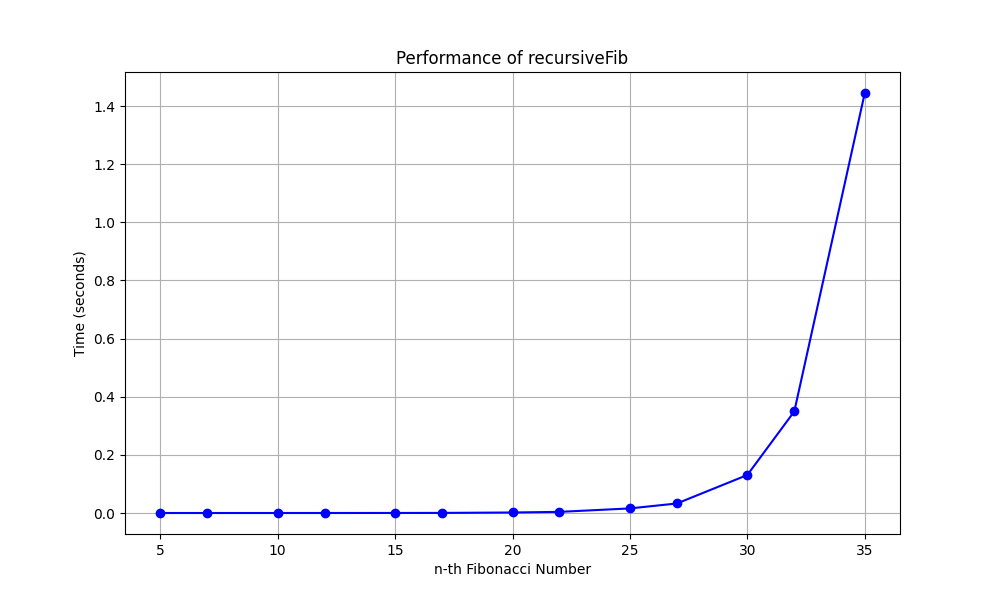
\includegraphics[width=.9\linewidth]{recursiveFib.png}
\label{orga327050}
\end{center}
\subsection{Memoized Recursive}
\label{sec:org8848356}
Memoization caches previously computed values to avoid redundant calculations.
\subsubsection{Implementation}
\label{sec:org4ffd122}
\begin{Code}
\begin{Verbatim}
\color{EFD}\EFk{def} \EFf{memoFib}(n, memo\textcolor[HTML]{000000}{=}\EFo{None}):
    \EFk{if} memo \EFk{is} \EFo{None}: memo \textcolor[HTML]{000000}{=} \{\}
    \EFk{if} n \textcolor[HTML]{000000}{<=} 1: \EFk{return} n
    \EFk{if} n \EFk{not} \EFk{in} memo:
        \EFv{memo}[n] \textcolor[HTML]{000000}{=} memoFib(n\textcolor[HTML]{000000}{-}1, memo) \textcolor[HTML]{000000}{+} memoFib(n\textcolor[HTML]{000000}{-}2, memo)
    \EFk{return} memo[n]
\end{Verbatim}
\end{Code}
\subsubsection{Results}
\label{sec:org7d2f43a}
As expected, we achieve T(n) time complexity:
\begin{Code}
\begin{Verbatim}
\color{EFD}plotFibPerformance(memoFib, input1)
\end{Verbatim}
\end{Code}

\begin{center}
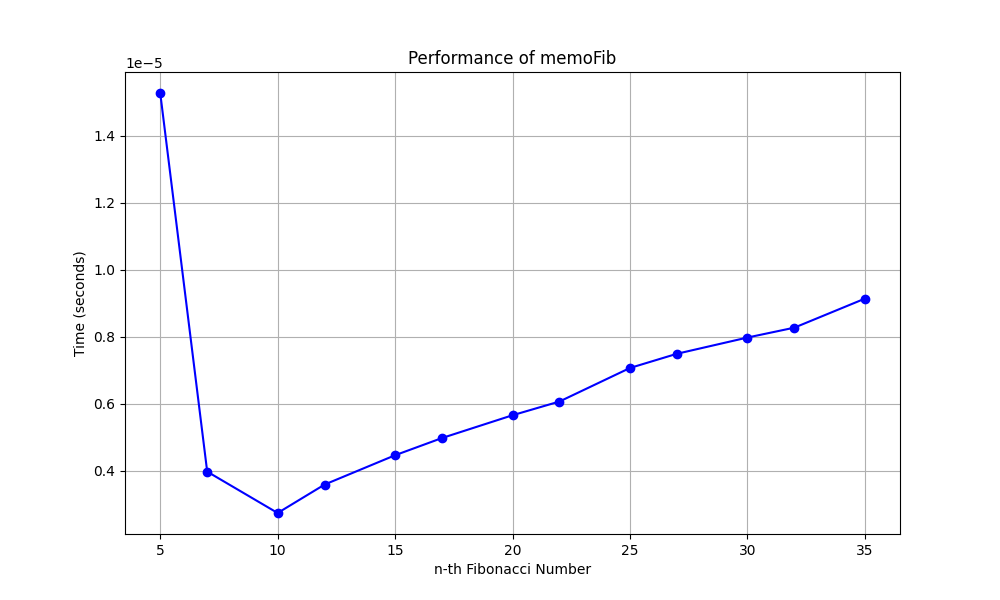
\includegraphics[width=.9\linewidth]{memoFib.png}
\label{org7880e48}
\end{center}
\subsection{Matrix Exponentiation}
\label{sec:org269d6fc}
The matrix exponentiation method computes Fibonacci numbers in T(log n) time by exploiting the relationship between consecutive Fibonacci numbers and matrix multiplication. The key insight is that:

\[ \begin{bmatrix} F_{n+1} & F_n \\ F_n & F_{n-1} \end{bmatrix} = \begin{bmatrix} 1 & 1 \\ 1 & 0 \end{bmatrix}^n \]

Therefore, \(F_n\) can be computed by raising the base matrix to the nth power using fast exponentiation.
\subsubsection{Implementation}
\label{sec:org88785a7}
This will allow us to deal with overflows
\begin{Code}
\begin{Verbatim}
\color{EFD}\EFv{MOD} \textcolor[HTML]{000000}{=} 10\textcolor[HTML]{000000}{**}9 \textcolor[HTML]{000000}{+} 7
\end{Verbatim}
\end{Code}

Function to multiply two 2x2 Matrices:
\begin{Code}
\begin{Verbatim}
\color{EFD}\EFk{def} \EFf{multiply}(A, B):
    \EFcd{\# }\EFc{Matrix to store the result}
    \EFv{C} \textcolor[HTML]{000000}{=} [[0, 0], [0, 0]]

    \EFcd{\# }\EFc{Matrix Multiply}
    C[0][0] \textcolor[HTML]{000000}{=} (A[0][0] \textcolor[HTML]{000000}{*} B[0][0] \textcolor[HTML]{000000}{+} A[0][1] \textcolor[HTML]{000000}{*} B[1][0]) \textcolor[HTML]{000000}{\%} MOD
    C[0][1] \textcolor[HTML]{000000}{=} (A[0][0] \textcolor[HTML]{000000}{*} B[0][1] \textcolor[HTML]{000000}{+} A[0][1] \textcolor[HTML]{000000}{*} B[1][1]) \textcolor[HTML]{000000}{\%} MOD
    C[1][0] \textcolor[HTML]{000000}{=} (A[1][0] \textcolor[HTML]{000000}{*} B[0][0] \textcolor[HTML]{000000}{+} A[1][1] \textcolor[HTML]{000000}{*} B[1][0]) \textcolor[HTML]{000000}{\%} MOD
    C[1][1] \textcolor[HTML]{000000}{=} (A[1][0] \textcolor[HTML]{000000}{*} B[0][1] \textcolor[HTML]{000000}{+} A[1][1] \textcolor[HTML]{000000}{*} B[1][1]) \textcolor[HTML]{000000}{\%} MOD

    \EFcd{\# }\EFc{Copy the result back to the first matrix}
    A[0][0] \textcolor[HTML]{000000}{=} C[0][0]
    A[0][1] \textcolor[HTML]{000000}{=} C[0][1]
    A[1][0] \textcolor[HTML]{000000}{=} C[1][0]
    A[1][1] \textcolor[HTML]{000000}{=} C[1][1]
\end{Verbatim}
\end{Code}

Function to find (Matrix \(M ^{expo}\))
\begin{Code}
\begin{Verbatim}
\color{EFD}\EFk{def} \EFf{power}(M, expo):
    \EFcd{\# }\EFc{Initialize result with identity matrix}
    \EFv{ans} \textcolor[HTML]{000000}{=} [[1, 0], [0, 1]]

    \EFcd{\# }\EFc{Fast Exponentiation}
    \EFk{while} expo:
        \EFk{if} expo \textcolor[HTML]{000000}{\&} 1:
            multiply(ans, M)
        multiply(M, M)
        \EFv{expo} \textcolor[HTML]{000000}{>>=} 1

    \EFk{return} ans
\end{Verbatim}
\end{Code}

And the fibonacci function per-ce:
\begin{Code}
\begin{Verbatim}
\color{EFD}\EFk{def} \EFf{matrixExpoFib}(n):
    \EFcd{\# }\EFc{Base case}
    \EFk{if} n \textcolor[HTML]{000000}{==} 0 \EFk{or} n \textcolor[HTML]{000000}{==} 1:
        \EFk{return} 1

    \EFv{M} \textcolor[HTML]{000000}{=} [[1, 1], [1, 0]]
    \EFcd{\# }\EFc{F(0) = 0, F(1) = 1}
    \EFv{F} \textcolor[HTML]{000000}{=} [[1, 0], [0, 0]]

    \EFcd{\# }\EFc{Multiply matrix M (n - 1) times}
    \EFv{res} \textcolor[HTML]{000000}{=} power(M, n \textcolor[HTML]{000000}{-} 1)

    \EFcd{\# }\EFc{Multiply Resultant with Matrix F}
    multiply(res, F)

    \EFk{return} res[0][0] \textcolor[HTML]{000000}{\%} MOD
\end{Verbatim}
\end{Code}
\subsubsection{Results}
\label{sec:orge0c26b6}
Here we measure the function, Roughly seeing the T(log n) complexity.
\begin{Code}
\begin{Verbatim}
\color{EFD}plotFibPerformance(matrixExpoFib, input2)
\end{Verbatim}
\end{Code}

\begin{center}
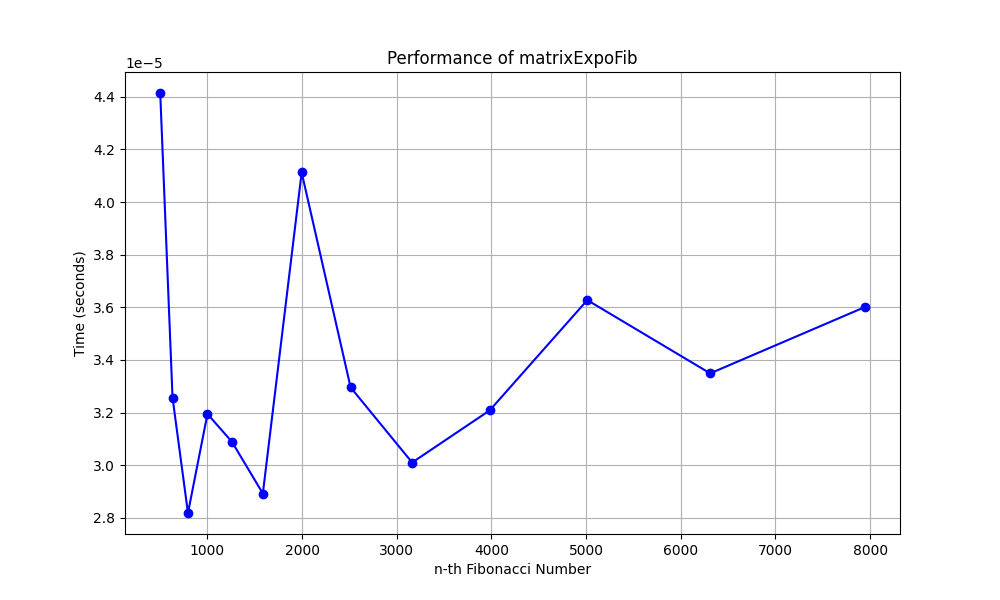
\includegraphics[width=.9\linewidth]{matrixExpoFib.png}
\label{org403c6f1}
\end{center}
\subsection{Fast Doubling method}
\label{sec:org889354d}
The Matrix Exponentiation Method is already discussed before. The Doubling Method can be seen as an improvement to the matrix exponentiation method to find the N-th Fibonacci number although it doesn’t use matrix multiplication itself.

The Fibonacci recursive sequence is given by 
\[
F(n+1) = F(n) + F(n-1)
\]

The Matrix Exponentiation method uses the following formula
The fast doubling method leverages the relationships between consecutive Fibonacci numbers using these identities:
\begin{align}
\label{eq:4}
F_{2n} = F_n(2F_{n+1} - F_n) \\
F_{2n+1} = F_{n+1}^2 + F_n^2
\end{align}
Like matrix exponentiation, this achieves T(log n) time complexity through recursive doubling.
\subsubsection{Implementation}
\label{sec:org3c4d57e}
\begin{Code}
\begin{Verbatim}
\color{EFD}\EFk{def} \EFf{fastDoublingFib}(n):
    \EFk{return} \_fib(n)[0]

\EFcd{\# }\EFc{Auxiliary method for Fast Doubling}
\EFk{def} \EFf{\_fib}(n):
    \EFk{if} n \textcolor[HTML]{000000}{==} 0:
        \EFk{return} 0, 1
    \EFk{else}:
        \EFv{a}, \EFv{b} \textcolor[HTML]{000000}{=} \_fib(n \textcolor[HTML]{000000}{//} 2)
        \EFv{c} \textcolor[HTML]{000000}{=} a \textcolor[HTML]{000000}{*} (b \textcolor[HTML]{000000}{*} 2 \textcolor[HTML]{000000}{-} a)
        \EFv{d} \textcolor[HTML]{000000}{=} a \textcolor[HTML]{000000}{*} a \textcolor[HTML]{000000}{+} b \textcolor[HTML]{000000}{*} b
        \EFk{if} n \textcolor[HTML]{000000}{\%} 2 \textcolor[HTML]{000000}{==} 0:
            \EFk{return} c, d
        \EFk{else}:
            \EFk{return} d, c \textcolor[HTML]{000000}{+} d
\end{Verbatim}
\end{Code}
\subsubsection{Results}
\label{sec:orgf333d80}
Here we measure the function. As expected, it is much faster than the matrix exponentiation method, whilst still having resemblence of the \(log(n)\) graph.
\begin{Code}
\begin{Verbatim}
\color{EFD}plotFibPerformance(fastDoublingFib, input2)
\end{Verbatim}
\end{Code}

\begin{center}
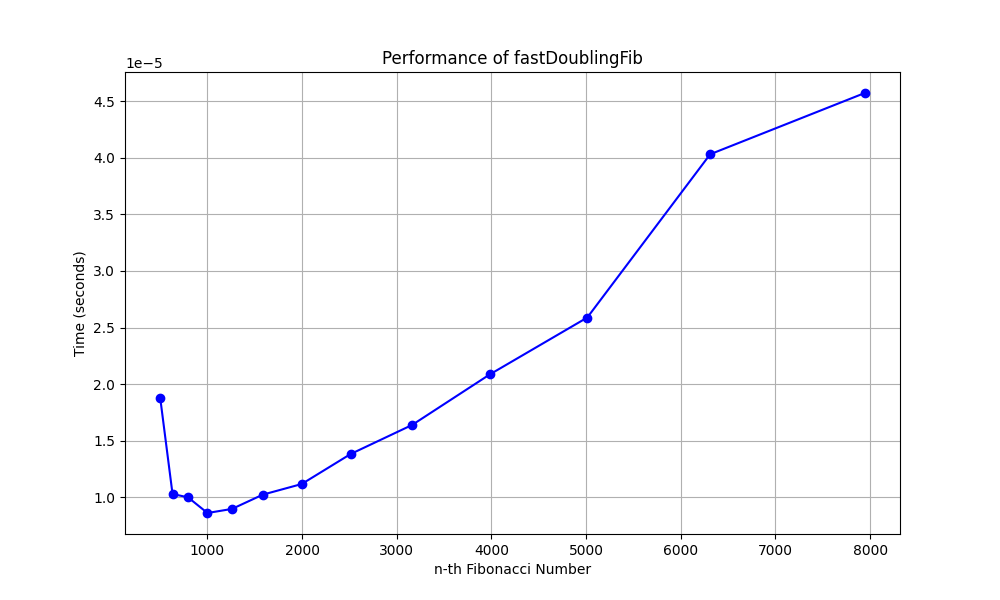
\includegraphics[width=.9\linewidth]{fastDoublingFib.png}
\label{orgdbd0233}
\end{center}
\subsection{Dinamic Programming}
\label{sec:org9cd461e}
The Dynamic Programming method, similar to the recursive method, takes the straightforward approach of calculating the n-th term. However, instead of calling the function upon itself, it stores just the previous two values. The recurrence relation is:
\[F_n = F_{n-1} + F_{n-2}\]
\subsubsection{Implementation}
\label{sec:org0ea12da}
\begin{Code}
\begin{Verbatim}
\color{EFD}\EFk{def} \EFf{dpFib}(n):
    \EFk{if} n \textcolor[HTML]{000000}{<=} 1: \EFk{return} n
    \EFv{a}, \EFv{b} \textcolor[HTML]{000000}{=} 0, 1
    \EFk{for} \_ \EFk{in} \EFb{range}(2, n \textcolor[HTML]{000000}{+} 1):
        \EFv{a}, \EFv{b} \textcolor[HTML]{000000}{=} b, a \textcolor[HTML]{000000}{+} b  \EFcd{\# }\EFc{Store only previous two values}
    \EFk{return} b
\end{Verbatim}
\end{Code}

This is optimal for computing a single Fibonacci number with respect to time complexity.
\subsubsection{Results}
\label{sec:org43a4f8e}
Showing excellent results with a time
complexity denoted in a corresponding graph of T(n):
\begin{Code}
\begin{Verbatim}
\color{EFD}plotFibPerformance(dpFib, input2)
\end{Verbatim}
\end{Code}

\begin{center}
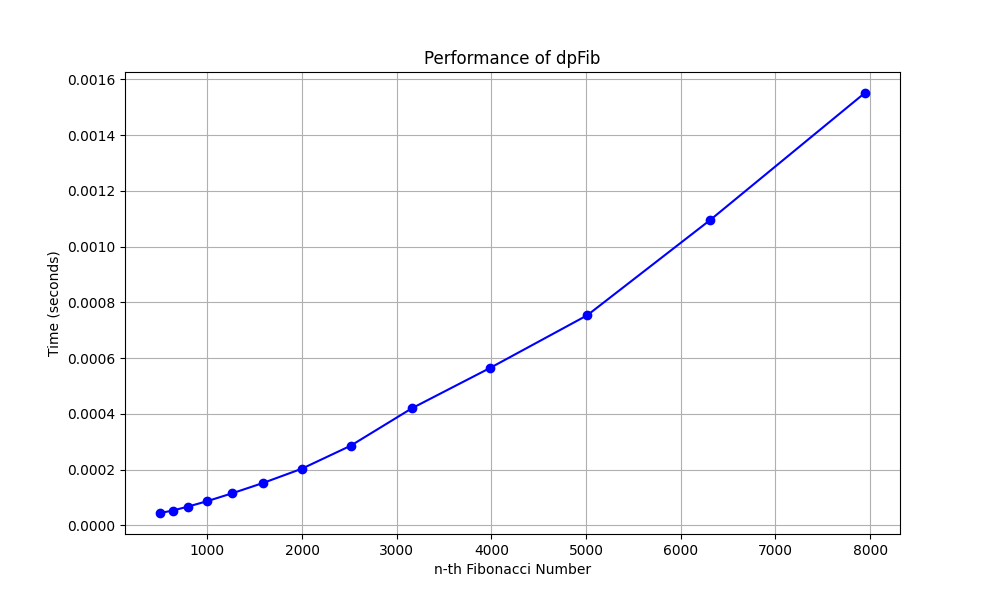
\includegraphics[width=.9\linewidth]{dinamicFib.png}
\label{org070cbde}
\end{center}
\subsection{Binet Formula Method}
\label{sec:org6de399f}
The Binet Formula Method is another unconventional way of calculating the n-th term of the
Fibonacci series, as it operates using the Golden Ratio formula, or phi. However, due to its nature of
requiring the usage of decimal numbers, at some point, the rounding error of python that accumulates,
begins affecting the results significantly.
\subsubsection{Implementation}
\label{sec:org4ce674d}
\begin{Code}
\begin{Verbatim}
\color{EFD}\EFk{import} math
\EFk{from} decimal \EFk{import} Decimal, Context, ROUND\_HALF\_EVEN


\EFv{input3} \textcolor[HTML]{000000}{=} [5, 7, 10, 12, 15, 17, 20, 22, 25, 27, 30, 32, 35, 47, 50, 55, 65, 70, 80, 100, 150, 166, 200]

\EFk{def} \EFf{binetFib}(n):
    \EFv{ctx} \textcolor[HTML]{000000}{=} Context(prec\textcolor[HTML]{000000}{=}60, rounding\textcolor[HTML]{000000}{=}ROUND\_HALF\_EVEN)
    \EFv{phi} \textcolor[HTML]{000000}{=} Decimal((1 \textcolor[HTML]{000000}{+} Decimal(5\textcolor[HTML]{000000}{**}(1\textcolor[HTML]{000000}{/}2))))
    \EFv{psi} \textcolor[HTML]{000000}{=} Decimal((1 \textcolor[HTML]{000000}{-} Decimal(5\textcolor[HTML]{000000}{**}(1\textcolor[HTML]{000000}{/}2))))
    \EFk{return} \EFb{int}((ctx.power(phi, Decimal(n)) \textcolor[HTML]{000000}{-} ctx.power(psi, Decimal(n))) \textcolor[HTML]{000000}{/} (2 \textcolor[HTML]{000000}{**} n \textcolor[HTML]{000000}{*} Decimal(5 \textcolor[HTML]{000000}{*} (1\textcolor[HTML]{000000}{/}2))))
\end{Verbatim}
\end{Code}
\subsubsection{Results}
\label{sec:orgb9708d8}
The errors starting with around 75-th number make the algorithm unusable in practice, despite its speed:
\begin{Code}
\begin{Verbatim}
\color{EFD}\EFv{numBinet} \textcolor[HTML]{000000}{=} binetFib(75)
\EFv{numDoubl} \textcolor[HTML]{000000}{=} fastDoublingFib(75)
\EFv{err} \textcolor[HTML]{000000}{=} \EFb{abs}(numBinet \textcolor[HTML]{000000}{-} numDoubl)
f\EFs{"binet:}\EFo{\char92{}t\char92{}t}\{numBinet\}\EFo{\char92{}n}\EFs{vs fast doubling:}\EFo{\char92{}t}\{numDoubl\}\EFo{\char92{}n}\EFs{The error:}\EFo{\char92{}t}\{err\}\EFs{"}
\end{Verbatim}
\end{Code}

\phantomsection
\label{org5e9c946}
\begin{verbatim}
binet:		1888569667134150
vs fast doubling:	2111485077978050
The error:	222915410843900
\end{verbatim}



And here is the performance graph:
\begin{Code}
\begin{Verbatim}
\color{EFD}plotFibPerformance(binetFib, input3)
\end{Verbatim}
\end{Code}

\begin{center}
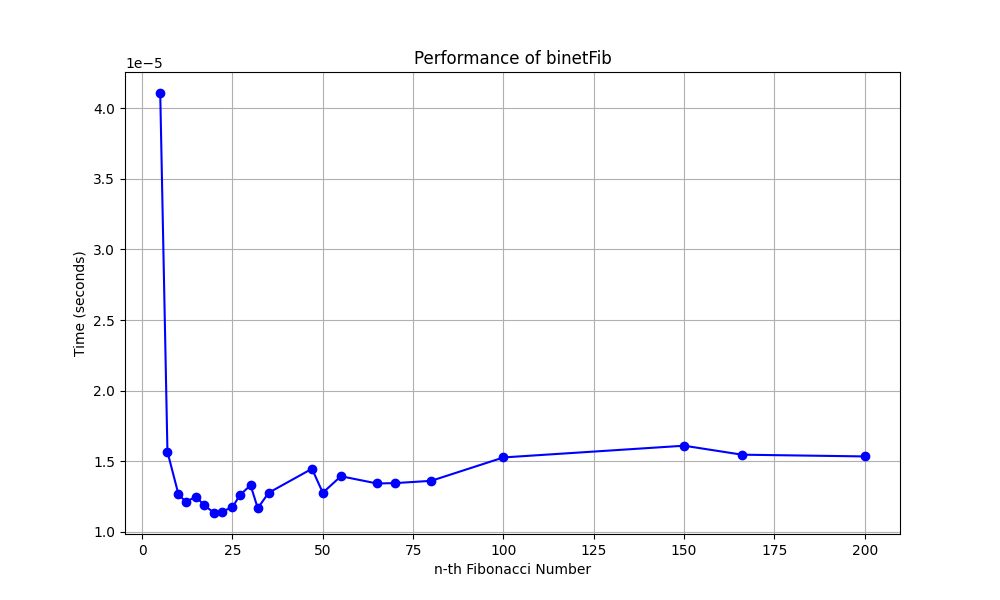
\includegraphics[width=.9\linewidth]{binetFormulaFib.png}
\label{org6ffa64d}
\end{center}
\section{Conclusions}
\label{sec:orgb7af16d}
In this laboratory, we analyzed various algorithms for calculating Fibonacci numbers, focusing on their empirical performance. Six distinct methods were implemented and tested: the Recursive Method, Memoized Recursive Method, Matrix Exponentiation, Fast Doubling Method, Dynamic Programming, and the Binet Formula. The main comparison metric was the execution time of each algorithm, measured across different input sizes.

The basic \textbf{\textbf{Recursive Method}} demonstrated poor performance as the input size increased due to its exponential time complexity of \(O(2^n)\). This inefficiency was evident in the execution times, particularly for larger values of n, where the algorithm required excessive computation due to recalculating the same Fibonacci numbers multiple times.

The \textbf{\textbf{Memoized Recursive Method}} showed significant improvement by storing previously computed values, which reduced the time complexity from \(O(2^n)\) to \(O(n)\). This method proved to be much faster and more efficient than the plain recursive approach, particularly when dealing with larger values of n.

The \textbf{\textbf{Matrix Exponentiation Method}} used matrix multiplication to calculate Fibonacci numbers in \(O(\log n)\) time. This logarithmic time complexity resulted in a considerable speedup compared to the recursive methods, and it was much faster for larger input sizes. The graph data confirmed the expected \(O(\log n)\) relationship between input size and execution time, making it a viable option for more extensive computations.

The \textbf{\textbf{Fast Doubling Method}} further optimized the matrix exponentiation approach by leveraging the relationships between consecutive Fibonacci numbers. Like matrix exponentiation, it achieved \(O(\log n)\) time complexity but outperformed it in terms of execution speed. This method was the most efficient for large input sizes, providing both faster execution and maintaining accuracy in the results.

The \textbf{\textbf{Dynamic Programming Method}} stored only the last two Fibonacci numbers at each step, which made it highly efficient. With \(O(n)\) time complexity and minimal space usage, this method performed excellently across all input sizes, being both fast and memory-efficient. It stands out as a reliable and optimal choice for computing Fibonacci numbers in practice.

Lastly, the \textbf{\textbf{Binet Formula}} provided a fast way to calculate Fibonacci numbers using the Golden Ratio. However, this method became unreliable for large input sizes due to rounding errors that accumulated as the Fibonacci numbers grew. While it demonstrated fast execution for smaller numbers, the lack of accuracy with larger n makes it unsuitable for practical applications at scale.

In conclusion, the \textbf{\textbf{Dynamic Programming}} and \textbf{\textbf{Fast Doubling}} methods emerged as the most efficient algorithms for calculating Fibonacci numbers, especially for large input sizes. The Memoized Recursive Method also offered a substantial improvement over the plain recursive method. Although the \textbf{\textbf{Matrix Exponentiation}} method is a strong candidate for moderately large Fibonacci numbers, \textbf{\textbf{Fast Doubling}} proved to be the best option overall in terms of both speed and accuracy. The \textbf{\textbf{Binet Formula}}, while fast, is not recommended for larger Fibonacci numbers due to its accuracy limitations.
\end{document}
